%==============================================================================
%  Recipe Box -- Technical Documentation
%  A Flask + SQLite personal recipe manager with Google Gemini AI helpers
%==============================================================================
\documentclass[11pt,a4paper]{article}

%------------------------------------------------------------------------------
% Packages
%------------------------------------------------------------------------------
\usepackage[utf8]{inputenc}
\usepackage[T1]{fontenc}
\usepackage{lmodern}
\usepackage[margin=2.4cm]{geometry}
\usepackage[dvipsnames,table]{xcolor}
\usepackage{graphicx}
\usepackage{booktabs}
\usepackage{longtable}
\usepackage{array}
\usepackage{tabularx}
\usepackage{enumitem}
\usepackage{listings}
\usepackage{caption}
\usepackage{titlesec}
\usepackage{fancyhdr}
\usepackage{tikz}
\usetikzlibrary{arrows.meta,positioning,shapes.geometric,fit,backgrounds}
\usepackage[colorlinks=true,linkcolor=RoyalBlue,urlcolor=RoyalBlue,
            citecolor=RoyalBlue,linktoc=all]{hyperref}

%------------------------------------------------------------------------------
% Style configuration
%------------------------------------------------------------------------------
\definecolor{codebg}{RGB}{248,246,242}
\definecolor{codekw}{RGB}{143,63,20}
\definecolor{codestr}{RGB}{74,124,89}
\definecolor{codecom}{RGB}{154,139,121}
\definecolor{accent}{RGB}{179,84,30}
\definecolor{headbg}{RGB}{244,227,211}

\captionsetup{font=small,labelfont=bf}

\titleformat{\section}{\Large\bfseries\color{accent}}{\thesection}{0.8em}{}
\titleformat{\subsection}{\large\bfseries\color{accent!80!black}}{\thesubsection}{0.7em}{}
\titleformat{\subsubsection}{\normalsize\bfseries}{\thesubsubsection}{0.6em}{}

\pagestyle{fancy}
\fancyhf{}
\fancyhead[L]{\small\itshape Recipe Box --- Technical Documentation}
\fancyhead[R]{\small\thepage}
\renewcommand{\headrulewidth}{0.4pt}

\lstdefinestyle{py}{
  language=Python,
  basicstyle=\ttfamily\small,
  keywordstyle=\color{codekw}\bfseries,
  stringstyle=\color{codestr},
  commentstyle=\color{codecom}\itshape,
  numbers=left,
  numberstyle=\tiny\color{codecom},
  numbersep=8pt,
  backgroundcolor=\color{codebg},
  frame=single,
  rulecolor=\color{codecom!40},
  breaklines=true,
  showstringspaces=false,
  tabsize=4,
  captionpos=b
}
\lstdefinestyle{txt}{
  basicstyle=\ttfamily\small,
  backgroundcolor=\color{codebg},
  frame=single,
  rulecolor=\color{codecom!40},
  breaklines=true,
  captionpos=b
}
\lstset{style=py}

\newcommand{\code}[1]{\texttt{#1}}

%------------------------------------------------------------------------------
% Title
%------------------------------------------------------------------------------
\title{\vspace{-1.5cm}\textbf{\color{accent}Recipe Box}\\[0.3em]
       \large Technical Documentation \& Architecture Report}
\author{Prepared for the \emph{recipie-box} project}
\date{\today}

%==============================================================================
\begin{document}
%==============================================================================

\begin{titlepage}
  \centering
  \vspace*{3cm}
  {\Huge\bfseries\color{accent} Recipe Box\par}
  \vspace{0.6cm}
  {\Large A Flask + SQLite Recipe Manager with Gemini AI Helpers\par}
  \vspace{1.2cm}
  {\large\itshape Technical Documentation and Architecture Report\par}
  \vfill
  \begin{tabular}{rl}
    \toprule
    \textbf{Document type}   & Software design documentation \\
    \textbf{Application}     & Recipe Box (\code{recipie-box}) \\
    \textbf{Stack}           & Python / Flask / SQLAlchemy / SQLite / Gemini \\
    \textbf{Version}         & 1.0 (as observed in source) \\
    \textbf{Date}            & \today \\
    \bottomrule
  \end{tabular}
  \vfill
  {\small This report describes the system as implemented in the repository
   source code at the time of writing.}
  \vspace*{1.5cm}
\end{titlepage}

\tableofcontents
\newpage

%==============================================================================
\section{Introduction}
%==============================================================================

\subsection{Purpose of this document}
This document provides a complete technical reference for \textbf{Recipe Box},
a personal recipe-management web application. It describes the system's goals,
architecture, data model, HTTP interface, AI integration, frontend behaviour,
configuration, deployment, and known limitations. It is intended for developers
who need to understand, maintain, extend, or reproduce the application.

\subsection{Audience}
\begin{itemize}[nosep]
  \item \textbf{Maintainers} extending the feature set or fixing defects.
  \item \textbf{Reviewers} assessing the design and code quality.
  \item \textbf{Operators} deploying and configuring the application.
  \item \textbf{New contributors} onboarding onto the codebase.
\end{itemize}

\subsection{Scope}
In scope: the Flask application, its three Python modules, Jinja2 templates and
stylesheets, the SQLite schema and Alembic migrations, and the Gemini AI helper
functions. Out of scope: the Google Gemini service itself, the SQLite engine
internals, and any future features not present in the source.

\subsection{Terminology}
\begin{description}[nosep,leftmargin=3.2cm]
  \item[Recipe] A stored dish with instructions, servings, optional photo,
        tags, rating, and cached AI results.
  \item[Ingredient line] A single structured ingredient (amount, unit, name)
        belonging to a recipe.
  \item[Tag] A short label shared across recipes via a many-to-many relation.
  \item[AI helper] A function in \code{ai\_helper.py} that calls Gemini.
\end{description}

%==============================================================================
\section{System Overview}
%==============================================================================

\subsection{What the application does}
Recipe Box is a server-rendered web application that lets a single user maintain
a personal collection of recipes. Beyond standard CRUD (create, read, update,
delete), it offers photo uploads, structured ingredients, tag-based organisation,
favourites, star ratings, a serving-count scaler, search and filtering, a
``filmstrip'' browsing view, and three AI-assisted features powered by Google
Gemini:

\begin{enumerate}[nosep]
  \item \textbf{Recipe auto-fill} --- on the Add page, the user types a dish
        title and Gemini returns a full published recipe which auto-fills the
        form.
  \item \textbf{Dish origin} --- one click returns the likely cultural origin
        and history of a dish.
  \item \textbf{Nutrition estimate} --- one click returns a per-serving estimate
        of calories, protein, carbohydrates, and fat.
\end{enumerate}

AI results are cached in the database so each recipe is queried at most once per
feature.

\subsection{Feature summary}
\begin{table}[h]
\centering
\small
\begin{tabularx}{\textwidth}{@{}lX@{}}
\toprule
\textbf{Feature} & \textbf{Description} \\
\midrule
Recipe CRUD        & Add, view, edit, and delete recipes (\code{/add}, \code{/recipe/<id>}, \code{/edit/<id>}, \code{/delete/<id>}). \\
Photo uploads      & PNG, JPG, JPEG, GIF, WebP; maximum 5\,MB; stored in \code{static/uploads/}. \\
Structured ingredients & Parallel amount / unit / name rows with a dynamic ``Add ingredient'' control. \\
Servings scaler    & Changing servings on the recipe page rescales ingredient amounts and nutrition client-side. \\
Search \& filtering & Partial-text search across title, instructions, tags, and ingredient names; tag filter; favourites filter. \\
Filmstrip view     & Cards with photos, ratings, and tag pills in a scrollable track, toggled against a compact list view. \\
Ratings            & 1--5 stars set via a dropdown; displayed as filled/empty stars. \\
Favourites         & Boolean bookmark toggled in place. \\
Pagination         & 9 recipes per page. \\
AI helpers         & Auto-fill, dish origin, and nutrition estimate; cached in the database. \\
\bottomrule
\end{tabularx}
\caption{Application feature summary.}
\end{table}

%==============================================================================
\section{Technology Stack}
%==============================================================================

\begin{table}[h]
\centering
\small
\begin{tabularx}{\textwidth}{@{}llX@{}}
\toprule
\textbf{Layer} & \textbf{Technology} & \textbf{Role} \\
\midrule
Language      & Python 3.10+            & Application logic (README recommends 3.10+). \\
Web framework & Flask                   & Routing, request handling, templating, sessions. \\
ORM           & Flask-SQLAlchemy        & Declarative models and query API over SQLAlchemy 2.x. \\
Migrations    & Flask-Migrate (Alembic) & Schema versioning. \\
Database      & SQLite                  & File-based store at \code{instance/recipes.db}. \\
AI            & \code{google-genai}, Gemini \code{gemini-2.5-flash} & Origin, nutrition, and auto-fill helpers. \\
Config        & \code{python-dotenv}    & Loads \code{.env} secrets into the environment. \\
Templating    & Jinja2                  & Server-side HTML rendering. \\
Frontend      & Vanilla JavaScript + custom CSS & Interactivity and styling (no JS framework). \\
Server        & Gunicorn                & WSGI server for production. \\
\bottomrule
\end{tabularx}
\caption{Technology stack.}
\end{table}

The runtime dependency set is intentionally small, as declared in
\code{requirements.txt}:

\begin{lstlisting}[style=txt,caption={requirements.txt}]
Flask
Flask-SQLAlchemy
python-dotenv
gunicorn
google-genai
\end{lstlisting}

%==============================================================================
\section{Architecture}
%==============================================================================

\subsection{Layered view}
Recipe Box follows a conventional server-rendered (multi-page) MVC-style
architecture. The browser requests a route; Flask dispatches to a view function;
the view uses SQLAlchemy models to read or write the SQLite database; a Jinja2
template renders HTML that is returned to the browser. Selected interactions
(auto-fill, rating, favourites, delete, origin, nutrition) use small JSON
endpoints called by vanilla JavaScript via \code{fetch()}.

\begin{figure}[h]
\centering
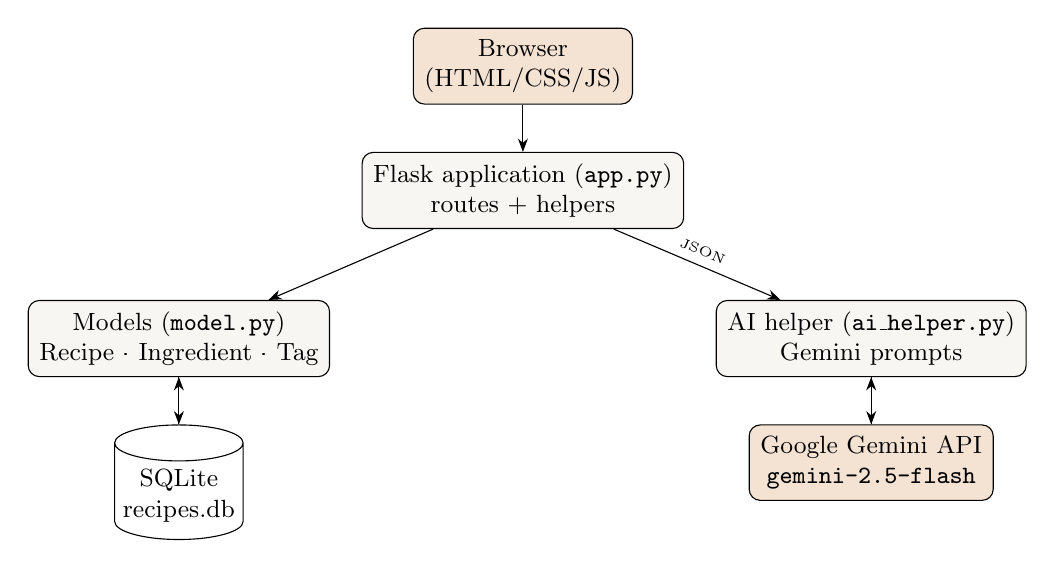
\begin{tikzpicture}[
  font=\small,
  node distance=6mm,
  box/.style={draw, rounded corners=4pt, align=center, minimum height=9mm,
              inner sep=4pt},
  store/.style={draw, cylinder, shape border rotate=90, aspect=0.28,
                align=center, minimum height=13mm, inner sep=3pt},
  >=Stealth
]
  \node[box, fill=headbg] (browser) {Browser\\(HTML/CSS/JS)};
  \node[box, fill=codebg, below=of browser] (flask)
      {Flask application (\code{app.py})\\routes + helpers};
  \node[box, fill=codebg, below left=9mm and 4mm of flask] (models)
      {Models (\code{model.py})\\Recipe · Ingredient · Tag};
  \node[box, fill=codebg, below right=9mm and 4mm of flask] (ai)
      {AI helper (\code{ai\_helper.py})\\Gemini prompts};
  \node[store, below=of models] (db) {SQLite\\recipes.db};
  \node[box, fill=headbg, below=of ai] (gemini) {Google Gemini API\\\code{gemini-2.5-flash}};

  \draw[->] (browser) -- (flask);
  \draw[->] (flask) -- (models);
  \draw[->] (flask) -- node[above,sloped]{\tiny JSON} (ai);
  \draw[->] (models) -- (db);
  \draw[->] (db) -- (models);
  \draw[->] (ai) -- (gemini);
  \draw[->] (gemini) -- (ai);
\end{tikzpicture}
\caption{Layered component architecture.}
\end{figure}

\subsection{Request lifecycle}
For a typical page request such as viewing a recipe:
\begin{enumerate}[nosep]
  \item The browser issues \code{GET /recipe/<id>}.
  \item Flask matches the route to \code{view\_recipe()}.
  \item The view calls \code{Recipe.query.get\_or\_404(id)}, loading the recipe
        and its related ingredient lines and tags from SQLite.
  \item \code{render\_template("recipe.html", recipe=recipe)} produces HTML.
  \item The browser renders the page; embedded JavaScript wires up the
        interactive controls and calls JSON endpoints on demand.
\end{enumerate}

\subsection{Code organisation}
\begin{table}[h]
\centering
\small
\begin{tabularx}{\textwidth}{@{}lX@{}}
\toprule
\textbf{Module} & \textbf{Responsibility} \\
\midrule
\code{app.py}        & Flask application object, configuration, route definitions, request helpers (image saving, tag resolution, ingredient parsing). \\
\code{model.py}      & SQLAlchemy \code{db} instance and the \code{Recipe}, \code{RecipeIngredient}, and \code{Tag} models plus the \code{recipe\_tags} association table. \\
\code{ai\_helper.py} & Gemini client, retry logic, JSON extraction, and the three AI feature functions. \\
\code{templates/}    & Jinja2 templates: \code{base.html}, \code{index.html}, \code{recipe.html}, \code{add.html}. \\
\code{static/}       & \code{style.css} and the \code{uploads/} directory for user photos. \\
\code{migrations/}   & Alembic environment and versioned migration scripts. \\
\code{instance/}     & Runtime SQLite database file. \\
\bottomrule
\end{tabularx}
\caption{Code organisation.}
\end{table}

%==============================================================================
\section{Data Model}
%==============================================================================

\subsection{Entity--relationship overview}
The schema has three entities and one association table:

\begin{itemize}[nosep]
  \item \textbf{Recipe} --- the central entity.
  \item \textbf{RecipeIngredient} --- one row per ingredient line (one-to-many
        from Recipe; cascade delete-orphan, ordered by id).
  \item \textbf{Tag} --- reusable label with a unique name.
  \item \textbf{recipe\_tags} --- many-to-many join between Recipe and Tag.
\end{itemize}

\begin{figure}[h]
\centering
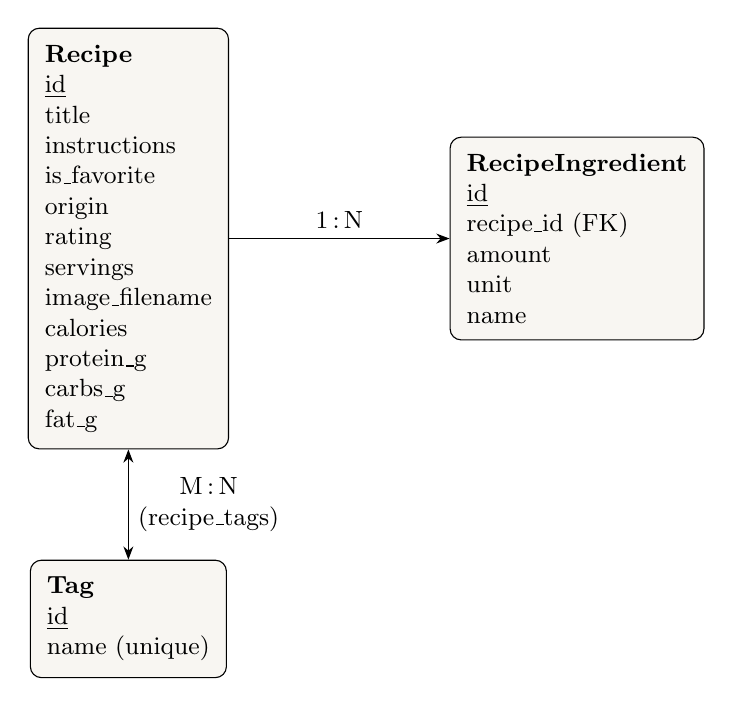
\begin{tikzpicture}[
  font=\small, node distance=10mm,
  entity/.style={draw, rounded corners=4pt, align=left, inner sep=6pt,
                 fill=codebg},
  >=Stealth
]
  \node[entity] (recipe)
    {\textbf{Recipe}\\\underline{id}\\title\\instructions\\is\_favorite\\origin\\rating\\servings\\image\_filename\\calories\\protein\_g\\carbs\_g\\fat\_g};
  \node[entity, right=28mm of recipe] (ing)
    {\textbf{RecipeIngredient}\\\underline{id}\\recipe\_id (FK)\\amount\\unit\\name};
  \node[entity, below=14mm of recipe] (tag)
    {\textbf{Tag}\\\underline{id}\\name (unique)};

  \draw[->] (recipe) -- node[above,align=center]{\small 1\,:\,N} (ing);
  \draw[<->] (recipe) -- node[right,align=center]{\small M\,:\,N\\(recipe\_tags)} (tag);
\end{tikzpicture}
\caption{Entity--relationship diagram.}
\end{figure}

\subsection{Table definitions}
\begin{longtable}{@{}p{3.4cm}p{3.3cm}p{1.3cm}p{6cm}@{}}
\toprule
\textbf{Table} & \textbf{Column} & \textbf{Type} & \textbf{Notes} \\
\midrule
\endfirsthead
\toprule
\textbf{Table} & \textbf{Column} & \textbf{Type} & \textbf{Notes} \\
\midrule
\endhead
\code{recipe} & id & Integer & Primary key. \\
              & title & String(120) & Not null. \\
              & instructions & Text & Not null. \\
              & is\_favorite & Boolean & Not null, default \code{False}. \\
              & origin & Text & Nullable; cached AI origin text. \\
              & rating & Integer & Nullable; 1--5. \\
              & servings & Integer & Not null, default 4. \\
              & image\_filename & String(200) & Nullable; uploaded photo filename. \\
              & calories & Integer & Nullable; cached AI estimate. \\
              & protein\_g & Integer & Nullable; cached AI estimate. \\
              & carbs\_g & Integer & Nullable; cached AI estimate. \\
              & fat\_g & Integer & Nullable; cached AI estimate. \\
\midrule
\code{recipe\_ingredient} & id & Integer & Primary key. \\
              & recipe\_id & Integer & Foreign key $\rightarrow$ \code{recipe.id}, not null. \\
              & amount & Float & Not null. \\
              & unit & String(20) & Nullable. \\
              & name & String(120) & Not null. \\
\midrule
\code{tag}    & id & Integer & Primary key. \\
              & name & String(50) & Not null, unique. \\
\midrule
\code{recipe\_tags} & recipe\_id & Integer & Composite primary key; FK $\rightarrow$ \code{recipe.id}. \\
              & tag\_id & Integer & Composite primary key; FK $\rightarrow$ \code{tag.id}. \\
\bottomrule
\caption{Database schema.}
\end{longtable}

\subsection{Model source excerpt}
\begin{lstlisting}[caption={model.py --- relationships and constraints (abridged)}]
recipe_tags = db.Table(
    "recipe_tags",
    db.Column("recipe_id", db.Integer, db.ForeignKey("recipe.id"), primary_key=True),
    db.Column("tag_id", db.Integer, db.ForeignKey("tag.id"), primary_key=True),
)

class Recipe(db.Model):
    id = db.Column(db.Integer, primary_key=True)
    title = db.Column(db.String(120), nullable=False)
    instructions = db.Column(db.Text, nullable=False)
    is_favorite = db.Column(db.Boolean, default=False, nullable=False)
    origin = db.Column(db.Text, nullable=True)
    rating = db.Column(db.Integer, nullable=True)
    servings = db.Column(db.Integer, default=4, nullable=False)
    image_filename = db.Column(db.String(200), nullable=True)

    calories = db.Column(db.Integer, nullable=True)
    protein_g = db.Column(db.Integer, nullable=True)
    carbs_g = db.Column(db.Integer, nullable=True)
    fat_g = db.Column(db.Integer, nullable=True)

    tags = db.relationship("Tag", secondary=recipe_tags, backref="recipes")
    ingredient_lines = db.relationship(
        "RecipeIngredient", backref="recipe",
        cascade="all, delete-orphan", order_by="RecipeIngredient.id"
    )
\end{lstlisting}

The \code{cascade="all, delete-orphan"} setting ensures that deleting a recipe
also removes its ingredient lines. Tag rows are shared and are \emph{not}
removed when a recipe is deleted; unreferenced tags may persist.

%==============================================================================
\section{Backend: Application Module (\texttt{app.py})}
%==============================================================================

\subsection{Configuration}
At import time the application sets:

\begin{lstlisting}[caption={Configuration constants}]
app.config["SQLALCHEMY_DATABASE_URI"] = "sqlite:///recipes.db"
app.config["SECRET_KEY"] = os.environ.get("SECRET_KEY", "dev-fallback-key-change-me")

UPLOAD_FOLDER = os.path.join("static", "uploads")
ALLOWED_EXTENSIONS = {"png", "jpg", "jpeg", "gif", "webp"}
MAX_FILE_SIZE = 5 * 1024 * 1024  # 5 MB
app.config["MAX_CONTENT_LENGTH"] = MAX_FILE_SIZE
RECIPES_PER_PAGE = 9
\end{lstlisting}

\subsection{Helper functions}
\begin{table}[h]
\centering
\small
\begin{tabularx}{\textwidth}{@{}lX@{}}
\toprule
\textbf{Helper} & \textbf{Behaviour} \\
\midrule
\code{allowed\_file(filename)} & Returns \code{True} if the file has a dot and its extension is in the allowed set. \\
\code{save\_uploaded\_image(file)} & Returns \code{None} if no file; \code{"INVALID"} if the type is rejected; otherwise saves the file under a random-prefixed secure name and returns that name. \\
\code{delete\_image\_file(filename)} & Removes the file from disk, ignoring missing files and \code{OSError}. \\
\code{get\_or\_create\_tags(string)} & Splits a comma-separated string, reuses existing \code{Tag} rows, and creates missing ones. \\
\code{parse\_ingredients\_from\_form()} & Zips the parallel \code{ing\_amount}/\code{ing\_unit}/\code{ing\_name} form lists into \code{RecipeIngredient} objects, skipping blank names. \\
\bottomrule
\end{tabularx}
\caption{Request helpers in \code{app.py}.}
\end{table}

\subsection{Route reference}
The following table is the normative HTTP interface of the application.

\begin{longtable}{@{}p{0.9cm}p{4.6cm}p{2.2cm}p{5.6cm}@{}}
\toprule
\textbf{Method} & \textbf{Path} & \textbf{Function} & \textbf{Description} \\
\midrule
\endfirsthead
\toprule
\textbf{Method} & \textbf{Path} & \textbf{Function} & \textbf{Description} \\
\midrule
\endhead
GET  & \code{/}                     & \code{home}            & Recipe list; supports \code{q}, \code{tag}, \code{favorites}, \code{page} query parameters. \\
GET  & \code{/recipe/<int:id>}      & \code{view\_recipe}    & Recipe detail page; 404 if not found. \\
GET/POST & \code{/add}             & \code{add\_recipe}     & Render the add form; on POST create the recipe and redirect home. \\
POST & \code{/api/recipe/suggest}   & \code{api\_recipe\_suggest} & JSON; fetch a published recipe for a title via Gemini. \\
GET/POST & \code{/edit/<int:id>}    & \code{edit\_recipe}    & Render the edit form; on POST update the recipe and clear cached nutrition. \\
POST & \code{/delete/<int:id>}      & \code{delete\_recipe}  & Delete the recipe and its photo, then redirect home. \\
POST & \code{/api/delete/<int:id>}  & \code{api\_delete\_recipe} & JSON delete used by the list view's \code{fetch} call. \\
POST & \code{/favorite/<int:id>}    & \code{toggle\_favorite} & Flip the favourite flag and redirect back. \\
POST & \code{/rate/<int:id>}        & \code{rate\_recipe}    & Validate and store a 1--5 rating. \\
POST & \code{/api/origin/<int:id>}  & \code{api\_recipe\_origin} & JSON; return cached or newly fetched dish origin. \\
POST & \code{/api/nutrition/<int:id>} & \code{api\_nutrition} & JSON; return cached or newly estimated nutrition. \\
\bottomrule
\caption{HTTP route reference.}
\end{longtable}

\subsection{Search and filtering}
The home route builds a SQLAlchemy query dynamically. When a search term is
present it performs outer joins to tags and ingredient lines and matches the
term case-insensitively against the title, instructions, tag name, and
ingredient name, then de-duplicates with \code{distinct()}:

\begin{lstlisting}[caption={Search query construction in \texttt{home()}}]
if search:
    pattern = f"%{search}%"
    query = query.outerjoin(Recipe.tags).outerjoin(
        Recipe.ingredient_lines
    ).filter(or_(
        Recipe.title.ilike(pattern),
        Recipe.instructions.ilike(pattern),
        Tag.name.ilike(pattern),
        RecipeIngredient.name.ilike(pattern),
    ))
    if tag:
        query = query.filter(Tag.name == tag)
    query = query.distinct()
elif tag:
    query = query.join(Recipe.tags).filter(Tag.name == tag)

if favorites_only:
    query = query.filter(Recipe.is_favorite == True)

pagination = query.order_by(Recipe.id.desc()).paginate(
    page=page, per_page=RECIPES_PER_PAGE, error_out=False
)
\end{lstlisting}

Results are ordered newest-first and paginated nine per page.

\subsection{AI result caching}
Both AI detail endpoints short-circuit when a cached value exists. The origin
endpoint returns the stored text immediately; the nutrition endpoint returns the
stored metrics and only calls Gemini when calories are still \code{None}. On
edit, the view resets \code{calories}, \code{protein\_g}, \code{carbs\_g}, and
\code{fat\_g} to \code{None} so nutrition is recomputed against the new
ingredient list.

\begin{lstlisting}[caption={Nutrition caching logic (abridged)}]
if recipe.calories is not None:
    return jsonify({"success": True, "calories": recipe.calories, ...})

if not recipe.ingredient_lines:
    return jsonify({"success": False,
                    "error": "No ingredients to estimate from."}), 400

result = get_nutrition_estimate(recipe.ingredient_lines, recipe.servings)
if result is None:
    return jsonify({"success": False,
                    "error": "Couldn't estimate nutrition right now."}), 500

recipe.calories = result.get("calories", 0)
# ... store protein, carbs, fat ...
db.session.commit()
\end{lstlisting}

%==============================================================================
\section{AI Integration (\texttt{ai\_helper.py})}
%==============================================================================

\subsection{Client and model}
A single module-level Gemini client is created from the \code{GEMINI\_API\_KEY}
environment variable, and requests target \code{gemini-2.5-flash}:

\begin{lstlisting}[caption={AI client setup}]
client = genai.Client(api_key=os.environ.get("GEMINI_API_KEY"))
MODEL = "gemini-2.5-flash"
TRANSIENT_STATUS_CODES = (429, 500, 503)
\end{lstlisting}

\subsection{Retry strategy}
\code{\_generate(prompt)} attempts the request up to three times. Transient
errors (HTTP 429, 500, 503) trigger a linear back-off of
\code{2\,$\times$\,(attempt+1)} seconds. All other exceptions propagate
immediately. If all attempts fail, the last error is raised.

\begin{lstlisting}[caption={Retry wrapper}]
def _generate(prompt):
    last_error = None
    for attempt in range(3):
        try:
            return client.models.generate_content(model=MODEL, contents=prompt)
        except Exception as e:
            last_error = e
            status = getattr(e, "code", None)
            if status not in TRANSIENT_STATUS_CODES:
                raise
            time.sleep(2 * (attempt + 1))
    raise last_error
\end{lstlisting}

\subsection{Robust JSON extraction}
The nutrition and auto-fill helpers expect JSON. Gemini sometimes wraps JSON in
markdown fences or adds prose, so \code{\_extract\_json()} first strips code
fences and then, failing a direct parse, extracts the substring from the first
\code{\{} to the last \code{\}}. It returns \code{None} when no valid object is
found.

\subsection{Feature functions}
\begin{table}[h]
\centering
\small
\begin{tabularx}{\textwidth}{@{}lX@{}}
\toprule
\textbf{Function} & \textbf{Behaviour} \\
\midrule
\code{get\_recipe\_origin(title)} & Asks Gemini for 3--4 factual sentences on the dish's likely origin; returns \code{"Unknown origin."} on failure. \\
\code{get\_nutrition\_estimate(lines, servings)} & Formats the structured ingredients, requests a strict JSON object of calories/protein/carbs/fat per serving, and returns the parsed dict or \code{None}. \\
\code{get\_recipe\_from\_web(title)} & Requests a genuine published recipe as JSON with title, servings, ingredients, instructions, and tags; applies defaults for any missing keys. \\
\bottomrule
\end{tabularx}
\caption{AI helper functions.}
\end{table}

The auto-fill prompt instructs Gemini to return only a JSON object and specifies
real quantities, \code{0} for non-numeric amounts, short single-word tags, and
complete instructions. The route layer additionally guards against duplicates:
if a recipe whose title matches the request already exists, the endpoint returns
HTTP \code{409} with \code{already\_exists: true}.

%==============================================================================
\section{Frontend}
%==============================================================================

\subsection{Templates}
\begin{table}[h]
\centering
\small
\begin{tabularx}{\textwidth}{@{}lX@{}}
\toprule
\textbf{Template} & \textbf{Content} \\
\midrule
\code{base.html}    & Shared document skeleton, Google Fonts, stylesheet link, site navigation, flash-message rendering, and the global delete handler. \\
\code{index.html}   & Search bar, filter pills, film/list view toggle, filmstrip of flashcards, compact recipe list, pagination, and filmstrip/pagination JavaScript. \\
\code{recipe.html}  & Recipe detail: photo, rating control, origin section, servings scaler, ingredient list, nutrition facts, instructions, and action bar; includes origin, scaling, and nutrition scripts. \\
\code{add.html}     & Add/edit form with basics, photo upload, dynamic ingredient rows, instructions, and the auto-fill script. \\
\bottomrule
\end{tabularx}
\caption{Jinja2 templates.}
\end{table}

\subsection{Client-side behaviour}
\begin{itemize}[nosep]
  \item \textbf{Delete} --- a delegated click handler in \code{base.html} calls
        \code{POST /api/delete/<id>} and removes the corresponding card and list
        item without a page reload.
  \item \textbf{Film/list toggle} --- \code{setView()} switches the display of
        the filmstrip and list and shows or hides the film controls.
  \item \textbf{Filmstrip navigation} --- previous/next buttons scroll the
        track; dot indicators are generated by \code{refreshFilmControls()} and
        kept in sync on scroll using \code{requestAnimationFrame}.
  \item \textbf{Drag-to-scroll} --- mouse drag on the film track scrolls it
        horizontally and suppresses the click that would otherwise follow a
        drag.
  \item \textbf{Servings scaler} --- on input, each ingredient amount is
        multiplied by \code{newServings / baseServings} and nutrition values are
        rescaled with the same factor.
  \item \textbf{Origin / nutrition} --- buttons disable themselves, call the
        matching JSON endpoint, and replace or populate the relevant section.
  \item \textbf{Auto-fill} --- the Add form posts the title to
        \code{/api/recipe/suggest} and populates servings, ingredients,
        instructions, and tags from the response, with status messages for
        success, duplicates, and errors.
\end{itemize}

\subsection{Styling and design system}
\code{static/style.css} defines a warm ``paper and ink'' palette through CSS
custom properties, including accent (\code{\#b3541e}), gold, green, cream
backgrounds, and shadow/radius tokens. Typography uses Fraunces for display,
Work Sans for body text, and IBM Plex Mono for code. The stylesheet is a plain
custom stylesheet with no framework dependency.

\begin{lstlisting}[style=txt,caption={Design tokens (excerpt)}]
--font-display: "Fraunces", Georgia, serif;
--font-body: "Work Sans", -apple-system, "Segoe UI", sans-serif;
--accent: #b3541e;
--accent-soft: #f4e3d3;
--gold: #d4a017;
--green: #4a7c59;
--radius: 18px;
\end{lstlisting}

%==============================================================================
\section{Security and Validation}
%==============================================================================

\begin{table}[h]
\centering
\small
\begin{tabularx}{\textwidth}{@{}lX@{}}
\toprule
\textbf{Area} & \textbf{Current control} \\
\midrule
Upload type      & Extension allow-list (png, jpg, jpeg, gif, webp) checked by \code{allowed\_file}. \\
Upload size      & Enforced by \code{MAX\_CONTENT\_LENGTH} (5\,MB) at the request level. \\
Upload filename  & Passed through \code{secure\_filename} and prefixed with 8 random bytes from \code{os.urandom} to prevent collisions and traversal. \\
Rating input     & Validated to be an integer in the range 1--5 before storage. \\
Secret key       & Read from the \code{SECRET\_KEY} environment variable with a development fallback. \\
\bottomrule
\end{tabularx}
\caption{Security and validation controls.}
\end{table}

\paragraph{Considerations.} The application currently has no authentication, so
every route is publicly reachable when deployed; it is intended for personal or
local use. Search inputs are bound as SQL parameters through SQLAlchemy. Auto-fill
output is inserted into the DOM via string templates in the browser, so if the
app is exposed to untrusted input, output escaping should be reviewed. The
development fallback secret key must not be used in production.

%==============================================================================
\section{Configuration and Environment}
%==============================================================================

Configuration is supplied through a \code{.env} file (gitignored), loaded by
\code{load\_dotenv()}.

\begin{table}[h]
\centering
\small
\begin{tabularx}{\textwidth}{@{}lXl@{}}
\toprule
\textbf{Variable} & \textbf{Purpose} & \textbf{Required} \\
\midrule
\code{SECRET\_KEY}     & Flask session signing key. & Recommended \\
\code{GEMINI\_API\_KEY} & Google AI Studio key used by \code{ai\_helper.py}. & For AI features \\
\bottomrule
\end{tabularx}
\caption{Environment variables.}
\end{table}

If \code{SECRET\_KEY} is unset the app falls back to a development value. If
\code{GEMINI\_API\_KEY} is unset, the AI client is created with a \code{None}
key; the app still starts, but AI calls fail and the corresponding endpoints
return error responses.

%==============================================================================
\section{Database Migrations}
%==============================================================================

Schema changes are managed with Flask-Migrate (Alembic). The repository contains
two revisions:

\begin{table}[h]
\centering
\small
\begin{tabularx}{\textwidth}{@{}llX@{}}
\toprule
\textbf{Revision} & \textbf{Revises} & \textbf{Change} \\
\midrule
\code{e706726d476a} & (base)          & Initial migration: creates \code{recipe} (with a \code{notes} column), \code{tag}, \code{recipe\_ingredient}, and \code{recipe\_tags}. \\
\code{2ce78e599d64} & \code{e706726d476a} & Removes the \code{notes} column from \code{recipe} using a batch alter. \\
\bottomrule
\end{tabularx}
\caption{Alembic migrations.}
\end{table}

After changing \code{model.py}, generate and apply a migration:

\begin{lstlisting}[style=txt,caption={Migration workflow}]
flask db migrate -m "description of change"
flask db upgrade
\end{lstlisting}

The \code{migrations/env.py} is the standard Flask-Migrate environment. It
resolves the engine through the Flask app's migration extension and configures
the target metadata so \code{autogenerate} can detect model changes. A
\code{process\_revision\_directives} hook suppresses empty migrations when no
schema changes are detected.

%==============================================================================
\section{Installation and Deployment}
%==============================================================================

\subsection{Prerequisites}
\begin{itemize}[nosep]
  \item Python 3.10 or newer.
  \item A Google AI Studio API key for the AI features.
\end{itemize}

\subsection{Setup}
\begin{lstlisting}[style=txt,caption={Local setup (Windows PowerShell)}]
python -m venv .venv
.venv\Scripts\activate
pip install -r requirements.txt

# create .env with SECRET_KEY and GEMINI_API_KEY

$env:FLASK_APP="app.py"
.venv\Scripts\python.exe -m flask db upgrade
.venv\Scripts\python.exe app.py        # http://127.0.0.1:5000
\end{lstlisting}

On macOS or Linux, activate with \code{source .venv/bin/activate} and run the
Python binary from \code{.venv/bin/}. For a debug server use
\code{python -m flask run --debug}.

\subsection{Production}
The README specifies Gunicorn as the production WSGI server:

\begin{lstlisting}[style=txt,caption={Production run}]
gunicorn app:app
\end{lstlisting}

Note that the SQLite database lives in \code{instance/recipes.db} and uploads
in \code{static/uploads/}; both must persist across restarts and be writable by
the serving process. A single-process deployment is advisable with SQLite.

%==============================================================================
\section{Repository Layout}
%==============================================================================

\begin{lstlisting}[style=txt,caption={Project tree (source only)}]
recipie-box/
  app.py                 # Flask app, routes, helpers, uploads
  model.py               # SQLAlchemy models and association table
  ai_helper.py           # Gemini calls: origin, nutrition, auto-fill
  requirements.txt
  README.md
  .env                   # secrets (gitignored)
  .gitignore
  static/
    style.css
    uploads/             # uploaded photos (gitignored)
  templates/
    base.html            # shared skeleton, nav, flashes, delete handler
    index.html           # list / filmstrip, search, filtering, pagination
    recipe.html          # detail + rating, scaler, origin, nutrition
    add.html             # add / edit form + auto-fill
  migrations/
    alembic.ini
    env.py
    script.py.mako
    versions/
      e706726d476a_initial_migration.py
      2ce78e599d64_remove_notes_field.py
  instance/
    recipes.db           # SQLite database (gitignored)
\end{lstlisting}

%==============================================================================
\section{Known Limitations and Future Work}
%==============================================================================

\begin{itemize}
  \item \textbf{No authentication or multi-user support} --- the app is
        single-user and all routes are open.
  \item \textbf{AI results are static once cached} --- origin text and nutrition
        are not versioned; nutrition is recomputed only when ingredients change
        on edit.
  \item \textbf{No test suite} --- correctness relies on manual verification;
        adding automated tests for helpers, routes, and \code{\_extract\_json}
        would improve confidence.
  \item \textbf{Ingredient amount parsing} --- a blank amount is stored as
        \code{0}; non-numeric amounts from the UI are constrained by the
        \code{number} input type.
  \item \textbf{Orphaned tags} --- deleting recipes leaves unreferenced
        \code{Tag} rows; a cleanup routine could prune them.
  \item \textbf{Upload validation} --- extension checks alone do not verify
        content; magic-byte validation would harden the upload path.
  \item \textbf{Client-side HTML construction} --- the nutrition and auto-fill
        scripts build markup with template strings; a DOM API approach would be
        safer against injection if input ever became untrusted.
  \item \textbf{Scalability} --- SQLite and a single Gunicorn worker are
        appropriate for personal use but not for concurrent multi-user load.
\end{itemize}

%==============================================================================
\section{Conclusion}
%==============================================================================

Recipe Box is a compact, well-structured Flask application that pairs a
conventional server-rendered CRUD core with a focused set of AI enhancements.
Its clear separation of concerns --- routing and helpers in \code{app.py}, the
data model in \code{model.py}, and Gemini access in \code{ai\_helper.py} ---
makes it straightforward to read and extend. Database caching of AI results and
a disciplined retry/JSON-extraction layer in the AI helper keep the external
dependency both economical and robust. The most valuable next steps are a test
suite, authentication if it is ever exposed beyond local use, and hardening of
the upload and client-rendered-content paths.

%==============================================================================
\appendix
\section{Appendix: Key Source Excerpts}
%==============================================================================

\subsection{Application bootstrap}
\begin{lstlisting}[caption={app.py --- imports and app setup}]
import os
from dotenv import load_dotenv
from flask import Flask, render_template, request, redirect, url_for, flash, jsonify
from flask_migrate import Migrate
from werkzeug.utils import secure_filename
from sqlalchemy import or_
from model import db, Recipe, Tag, RecipeIngredient
from ai_helper import get_recipe_origin, get_nutrition_estimate, get_recipe_from_web

load_dotenv()

app = Flask(__name__)
app.config["SQLALCHEMY_DATABASE_URI"] = "sqlite:///recipes.db"
app.config["SECRET_KEY"] = os.environ.get("SECRET_KEY", "dev-fallback-key-change-me")

db.init_app(app)
migrate = Migrate(app, db)
\end{lstlisting}

\subsection{Image upload helper}
\begin{lstlisting}[caption={app.py --- save\_uploaded\_image}]
def save_uploaded_image(file):
    if not file or file.filename == "":
        return None
    if not allowed_file(file.filename):
        flash("Image must be a png, jpg, jpeg, gif, or webp file.", "error")
        return "INVALID"
    filename = secure_filename(file.filename)
    unique_filename = f"{os.urandom(8).hex()}_{filename}"
    filepath = os.path.join(app.config["UPLOAD_FOLDER"], unique_filename)
    file.save(filepath)
    return unique_filename
\end{lstlisting}

\subsection{Glossary}
\begin{description}[nosep,leftmargin=3.4cm]
  \item[CRUD] Create, read, update, delete.
  \item[ORM] Object-relational mapping.
  \item[WSGI] Web Server Gateway Interface, the Python web server contract.
  \item[Jinja2] The Python templating engine used by Flask.
  \item[Alembic] The database migration tool used by Flask-Migrate.
  \item[Gemini] Google's generative AI model family used for the AI features.
  \item[Filmstrip] The horizontally scrolling card view of recipes.
\end{description}

\end{document}
